\section{Relay Attack Analysis}
\label{sec:problemStatement}

In this section, we provide an analysis of relay attacks on SGX. 

\begin{figure}[t]
 \centering
  %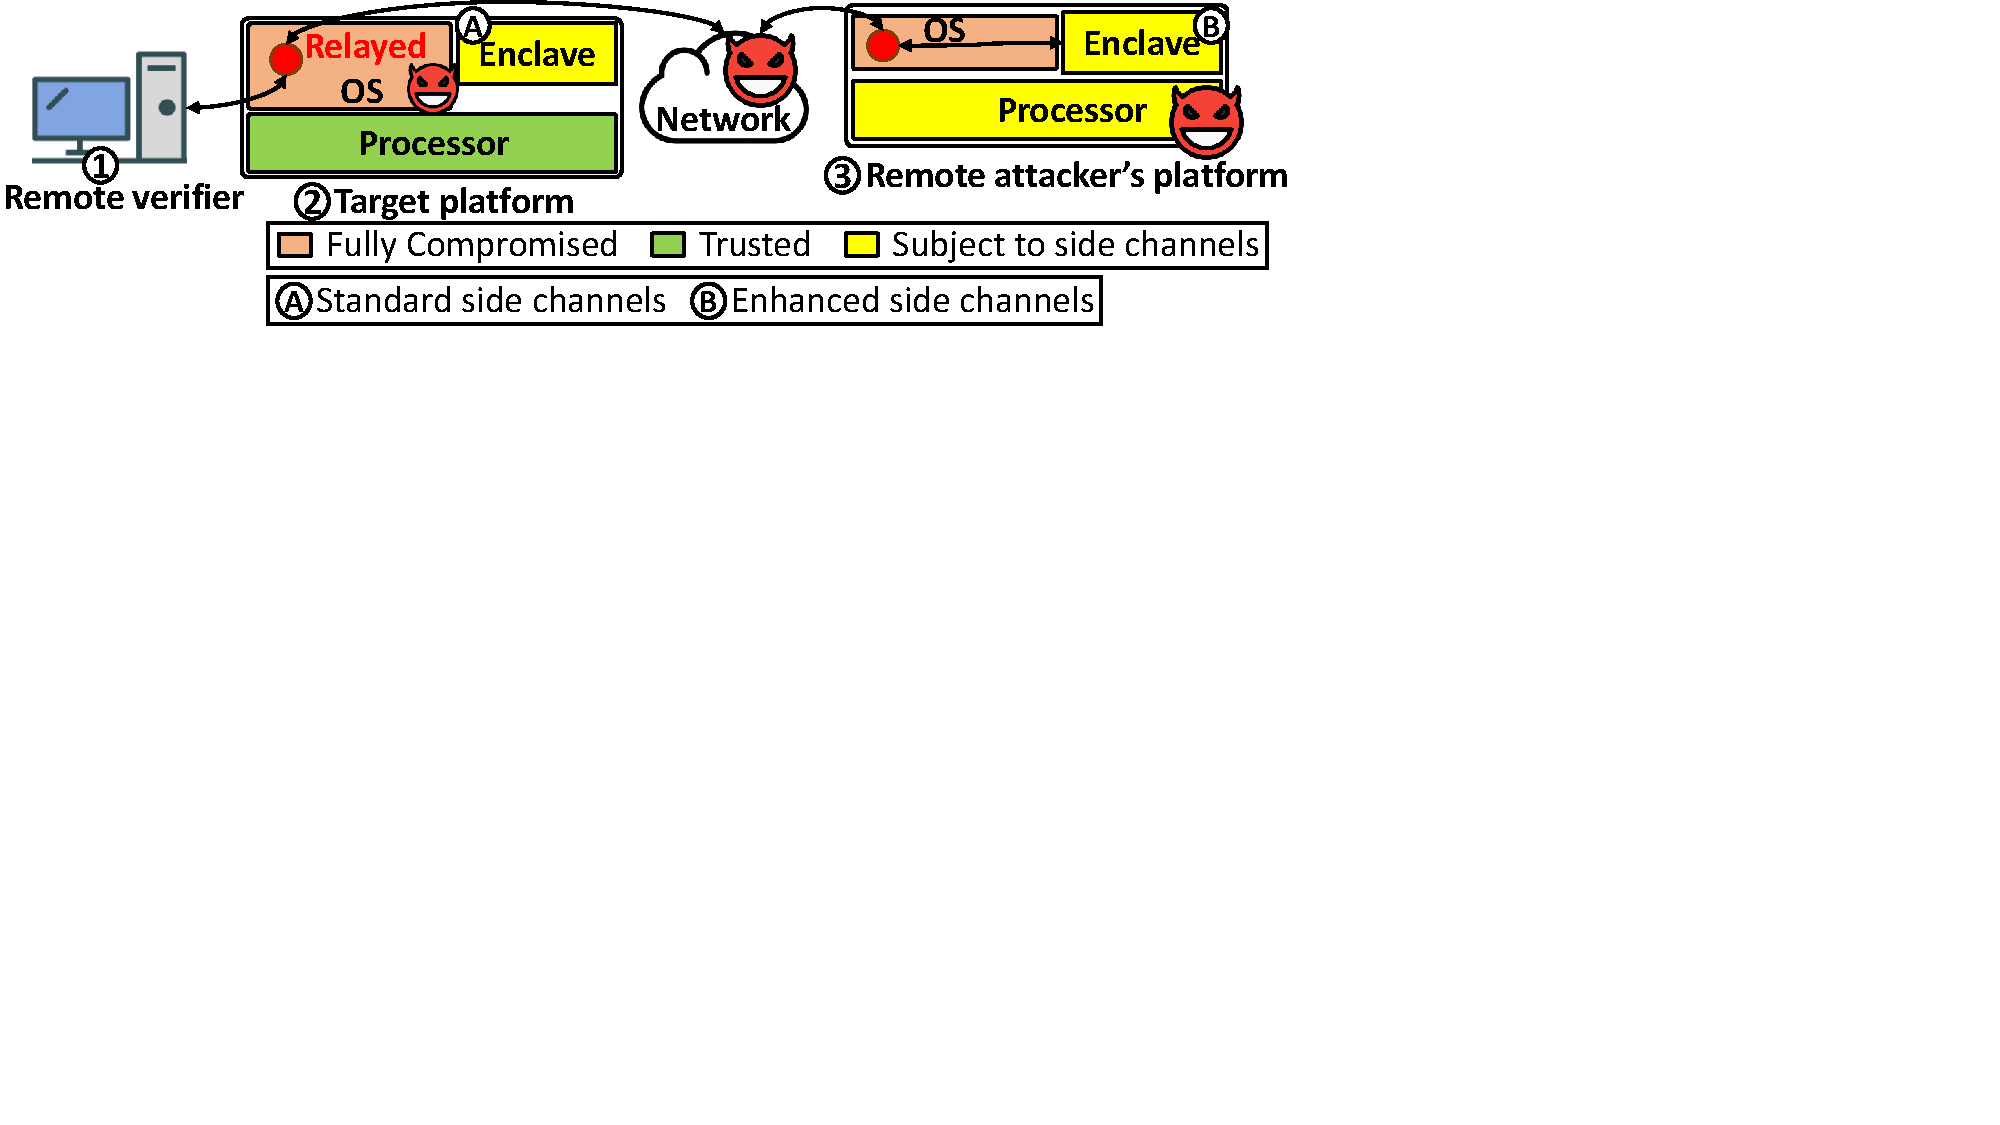
\includegraphics[trim={0 13.4cm 11cm 0},clip,width=\linewidth]{relayAttack.pdf}
  %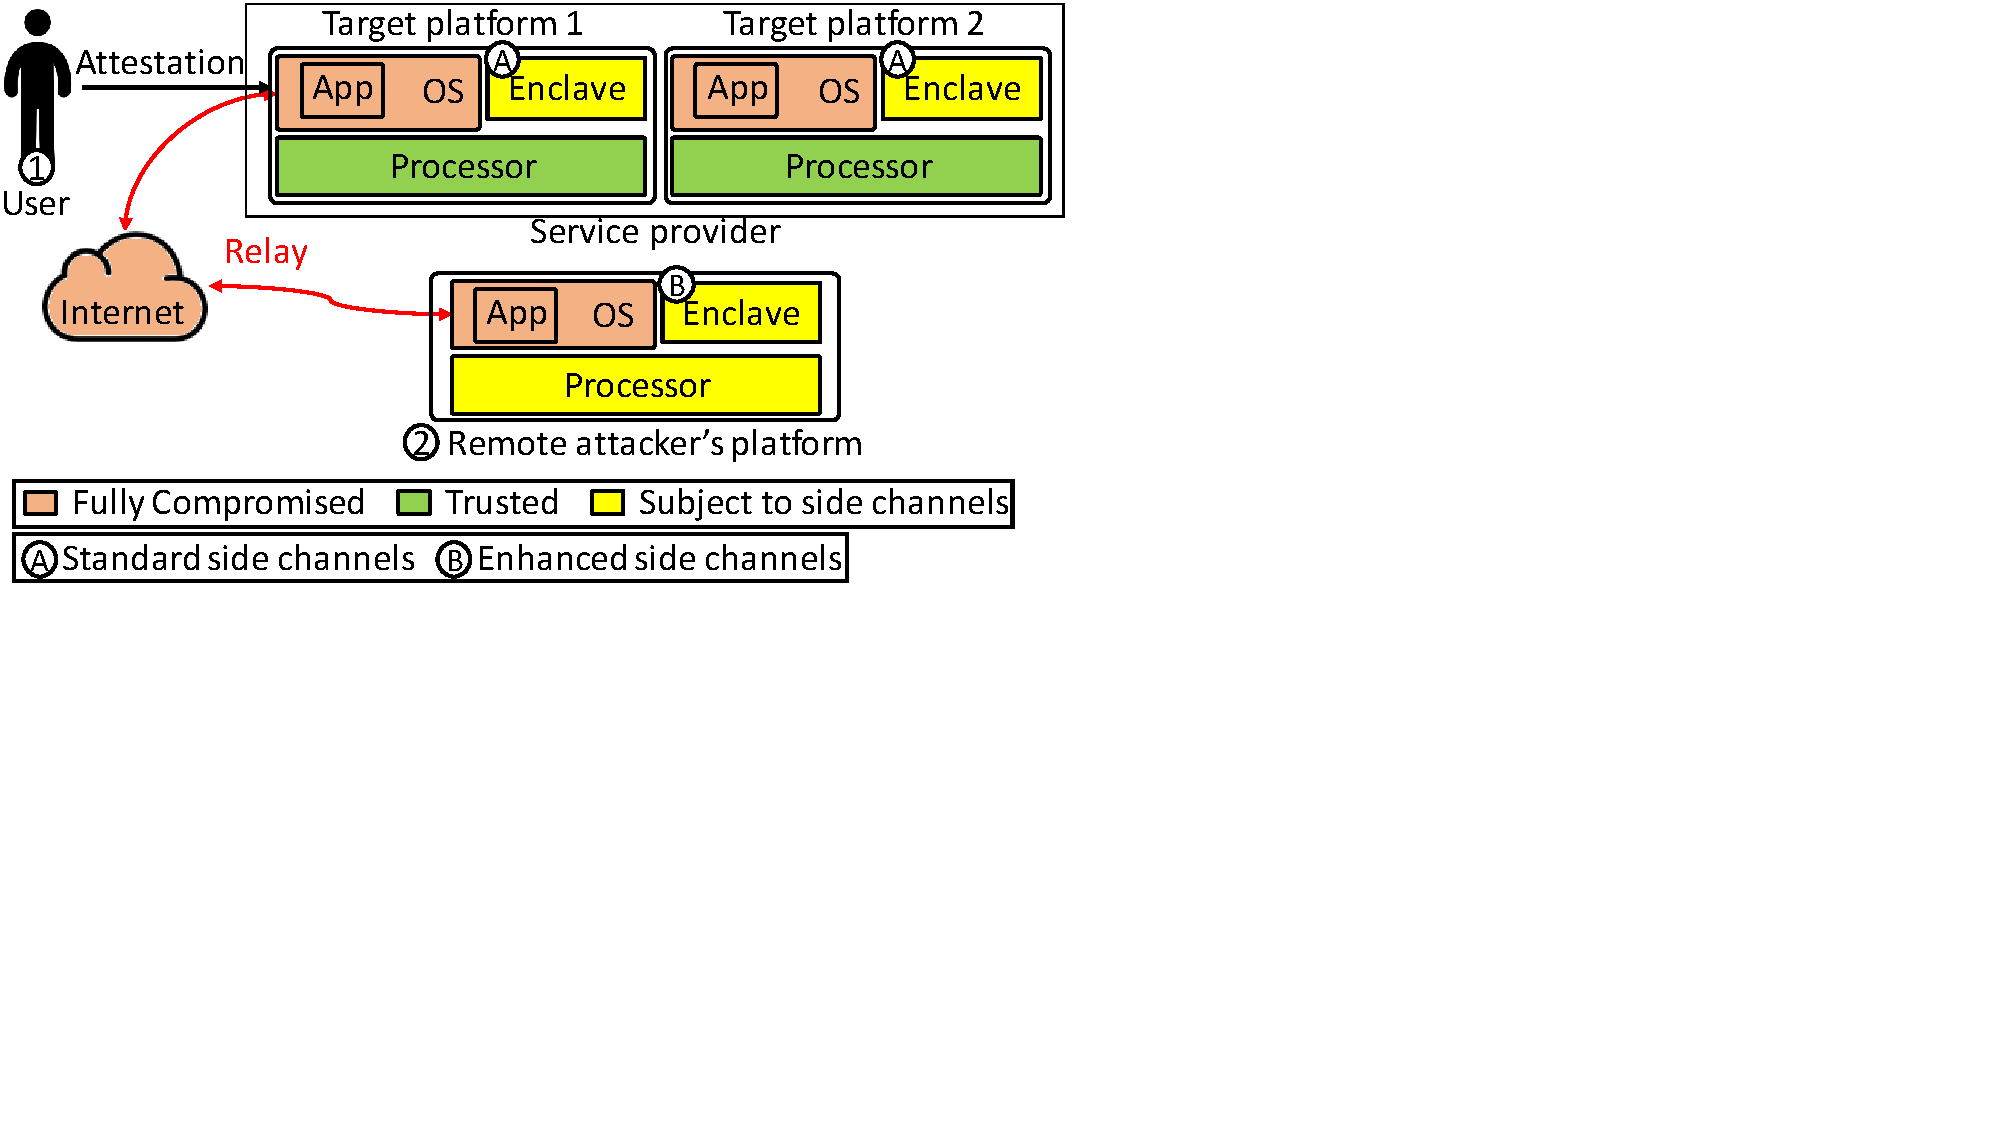
\includegraphics[trim={0cm 9cm 15.8cm 0},clip,width=0.75\linewidth]{chapters/ProximiTEE/figures/relayAttack2.pdf}
  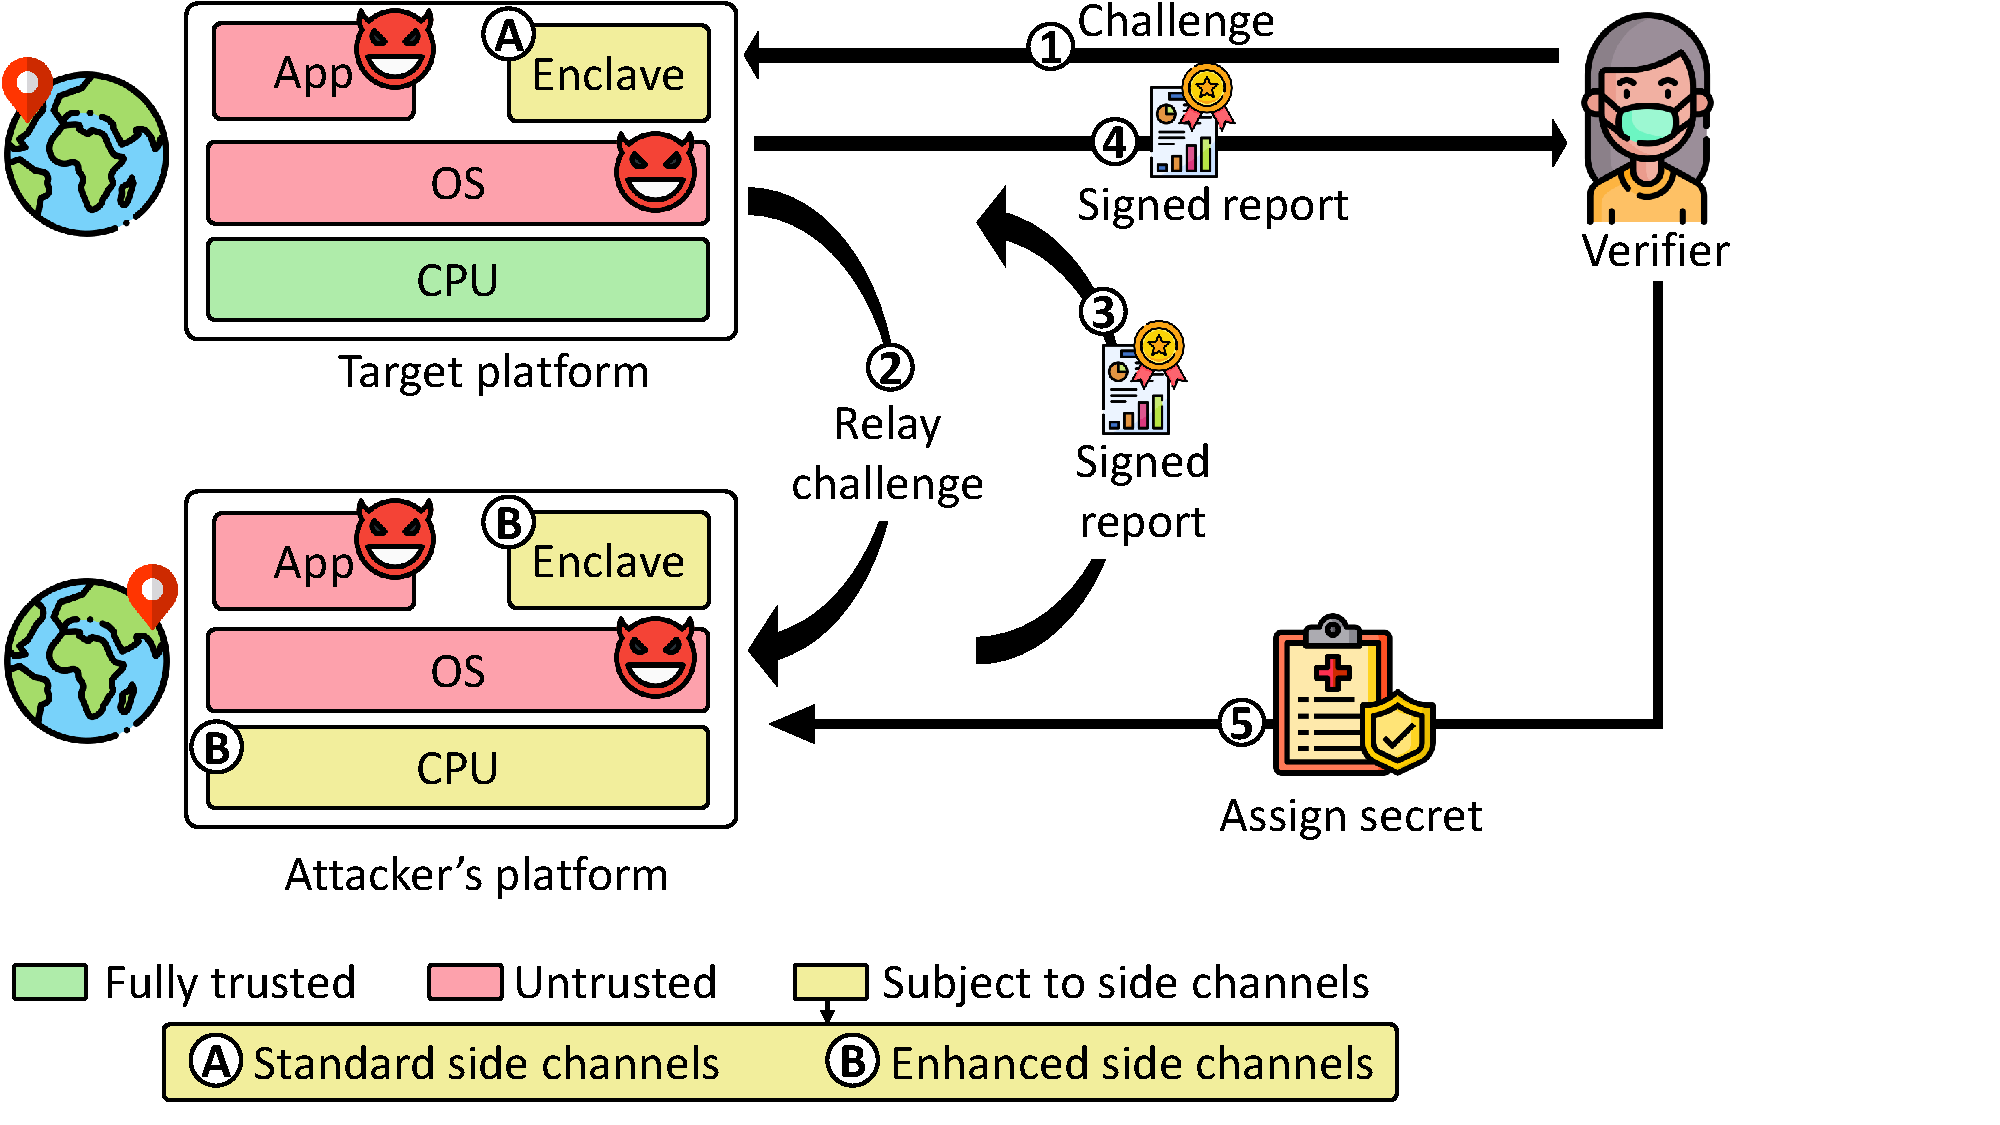
\includegraphics[trim={0 0 4.5cm 0},clip,width=0.9\linewidth]{chapters/ProximiTEE/images_new/relay.pdf}
 \caption[Relay attack]{\textbf{Relay attack.} The attacker redirects attestation to his own platform which gives him increased (side-channel and kernel-level) abilities to attack the attested enclave.}

 \label{fig:SystemModel}
\end{figure}


\subsection{Relay Attacks}
\label{sec:problemStatement:systemAttackerModel}

We consider a system model shown in Figure~\ref{fig:SystemModel} that consists of three parties: the target platform, the remote verifier, and the attacker's platform. The remote verifier is a trusted party that wishes to connect and attest to a specific SGX platform. The target platform is the SGX platform to which the remote verifier intends to connect. Finally, the attacker's platform is a platform owned by the attacker, connected to the target platform through the Internet.



\myparagraph{Attacker model} We consider the following attacker model that we call the \emph{relay attacker}. The relay attacker controls the OS and all other privileged software on the \emph{target} platform at least \emph{temporarily}, particularly at the time of the remote attestation. The OS compromise on the target platform maybe later detected and disinfected. We consider the case in which the target platform resides in a data center or otherwise in a facility with restricted physical access. Hence, the attacker hence \emph{does not} have physical access to the target platform (or any other co-located platform in the same facility). %The relay attacker cannot extract attestation or sealing keys from the target platform.

The relay attacker controls the OS and all other privileged software on the attacker's platform \emph{permanently} and has physical access to that platform. The attacker also controls the network between the target platform and his platform. At the time of the attestation, the attacker has not been able to extract attestation or sealing keys from his platform or any other SGX processor.


\myparagraph{The process of the relay attack} The relay attacker can redirect the attestation requests intended for the target platform to his platform, as shown in Figure~\ref{fig:SystemModel}. This is a realistic attack for two reasons. First, in the SGX attacker's model, the attacker can control the OS and, hence, easily redirect any network request the target platform receives. Second, even if the attacker cannot compromise the OS in the target platform, it might be able to exploit some vulnerability of the untrusted application managing the enclave. The exploit might allow the attacker to manipulate the application's control flow to redirect attestation requests to any platform he desires.




\begin{figure}[t]
\footnotesize
    \centering
    \begin{tikzpicture}[
solved/.style={rectangle,draw,fill=purple!40, rounded corners, align=center},
not/.style={rectangle, draw,fill=orange!60, rounded corners, align=center},
neutral/.style={rectangle, draw, rounded corners, align=center, fill=black!5},
sibling distance=12em]]
    \node[neutral](root) {SGX attacks}
    child { node[not, yshift=13pt] (name) {Attacks enabled by \\ leaked attestation keys ~\cite{foreshadow-usenix18}} }
    child { node[neutral, yshift=13pt, xshift=10pt] (app) {Side-Channels \\ on application enclave}
      child { node[neutral, yshift=0pt] (soft) {Software/digital}
		child { node[solved, yshift=-10pt] (pe) {Privilege\\ escalation}}      
        child { node[not, right=1.5em of pe,yshift=-10pt] (a) {Case (A) in Figure~\ref{fig:timeLine}:\\Complement of Case (B)}}
        child { node[solved, right=1.5em of a, yshift=-12pt] {Case (B) in Figure~\ref{fig:timeLine}:\\
            \begin{tabular}{rl}
                Target platform:& secure\\
                Attacker's platform:& vulnerable\\
            \end{tabular}}} }
      child { node[solved, yshift=12pt] (physical) {Physical} } };
      
    %\node[below=0cm of name] {Foreshadow~\cite{foreshadow-usenix18}};
    \node[below=0cm of physical](power) {Power analysis~\cite{wang2006covert}};
    \node[below=-5pt of power](EM) {EM radiation~\cite{gandolfi2001electromagnetic}};
    \node[below=-5pt of EM](ac) {Acoustic~\cite{shamir2004acoustic}};
         
    \node[left=10pt of soft](page) {Page fault~\cite{xu2015controlled}};
    \node[above=-3pt of page](cache) {Cache~\cite{dall2018cachequote,gotzfried2017cache,sgxcache,moghimi2017cachezoom}};
    \node[below=-2pt of page](branch) {Branch prediction~\cite{lee2017inferring}};
    %\node[below=-5pt of branch](synch) {Synchronization~\cite{asyncshock}};
      
    \node[solved, right=4em of root,  minimum size=3mm](l1) {};
    \node[right=0cm of l1](l1_1) {Enabled by relay};
    \node[not, below=1pt of l1, minimum size=3mm](l2) {};
    \node[right=0cm of l2](l2_1) {Independent of relay};
    
    \end{tikzpicture}
    
    \caption[Relay attack implications]{\textbf{Relay attack implications.} The tree shows the types of attacks that are enabled by  redirection and ones that are independent of relay.}
    \label{fig:relayTree}
\end{figure}

            
\subsection{Relay Attack Implications}
\label{sec:problemStatement:implication}

Although relay attacks have been known for a long time~\cite{parno2008bootstrapping}, their implications to modern TEEs like SGX have not been carefully analyzed. Next, we perform the first such analysis.

The main consequence of attestation redirection is that it \emph{increases the attacker's ability to attack the attested enclave} through side-channels which are a well-known limitation of SGX (see Section~\ref{sec:background:attacks}). In Figure~\ref{fig:relayTree} we highlight two major classes of attacks: those that are only possible by first performing a relay attack, which we denote as ``enabled by relay'', and those that can be done whether or not the attacker also executes a relay attack, which we call ``independent of relay.''


\myparagraph{Attacks using leaked attestation keys} Our first observation is that attacks are based on leaked attestation keys (e.g., ones obtained through the Foreshadow attack~\cite{foreshadow-usenix18}) are independent of relaying. If the attacker has obtained a valid and non-revoked attestation key, he can emulate an SGX processor on the target platform and obtain any secrets provisioned to it.


\myparagraph{Physical side channels} One major benefit of the relay, from the attacker's point of view, is that it enables \emph{physical} side-channel attacks against application enclaves. Once a secret has been provisioned to the attacker's platform, she has as much time as she likes to perform the attack. Some examples of physical side-channel attacks are acoustic, electric, and electromagnetic monitoring, which has been shown to be both effective and inexpensive means to extract secrets from modern PC platforms (see~\cite{genkin2016physical} for a summary of known attacks). Since the attacker does not have physical access to the target platform, such attacks are clearly not possible without a relay. Hardening programs like enclaves against physical side channels is difficult and currently an open problem~\cite{genkin2016physical}. Therefore, developers cannot easily defend their enclaves against physical side channels that are enabled by attestation redirection.


\myparagraph{Privilege escalation for digital side channels}
Another possible benefit of relay attacks is that it may enable \emph{privilege escalation}. In cases where the attacker has only compromised the user-space application that manages the enclave and not the OS, the application can redirect the attestation to the attacker's remote platform where he controls the OS as well. In such cases, the relay enables \emph{digital} side-channel attacks that require system privileges. Several such attacks have been recently demonstrated against SGX~\cite{moghimi2017cachezoom, sgxcache, gotzfried2017cache}.


\begin{figure}[t]
\footnotesize
    \centering
    \begin{tikzpicture}[
    solved/.style={rectangle,draw,fill=purple!40, rounded corners, align=center},
    relayNode/.style={circle,draw,fill=red!40, align=center},
    edge from parent/.style={draw,-latex},    
    neutral/.style={rectangle, draw, rounded corners, align=center, fill=black!5},
    not/.style={rectangle, draw,fill=orange!60, rounded corners, align=center},
    sibling distance=12em]]
    
 
 
 \node[] (targetA) {\textbf{Target}};
 \node[right=33pt of targetA] (attackA) {\textbf{Attacker}};
 \node[below=0 of attackA] (dummy) {};
 
  
 \node[neutral, below=0.1cm of targetA](root1) {OS compromised};    
 \node[relayNode, below = 1em of root1] (relay1) {Relay};
 \node[neutral, right = 3em of relay1] (attestation1) {Attest enclave};
 \node[neutral, below = 1em of relay1] (discovery1) {New attack\\ discovery};        
  \node[neutral, below = 2.2em of attestation1] (discoveryAttack1) {New attack\\ discovery};  
 \node[neutral, below = 0.6em of discoveryAttack1] (provisioning1) {Secret\\ provisioning};
 \node[neutral, below = 3.5em of discovery1] (cleanup1) {OS cleanup};    
 \node[below = 3em of cleanup1] (end) {};      
 \node[not, below = 2em of provisioning1] (independent) {Independent of relay};
 
 
  \draw[->, thick] (root1) edge[] node{} (relay1);
 \draw[->, thick] (relay1) edge[] node{} (discovery1);
 \draw[->, thick] (relay1) edge[] node{} (attestation1);
 \draw[->, thick] (attestation1) edge[] node{} (discoveryAttack1);
 \draw[->, thick] (discovery1) edge[] node{} (cleanup1); 
 \draw[->, thick] (discoveryAttack1) edge[] node{} (provisioning1);
 \draw[->, thick] (provisioning1) edge[] node{} (independent);
 \draw[->, thick] (dummy) edge[] node{} (attestation1);
 \draw[->, thick] (cleanup1) edge[] node{} (end);
  \node[below=0cm of independent] {Case (A)};
 

 \node[right=0.79cm of attackA](point1){};
 \node[below=19em of point1](point2){Time};
 \draw[->] (point1) edge[] node{} (point2);
 
 \node[right=50pt of attackA] (targetB) {\textbf{Target}};
 \node[right=37pt of targetB] (attackB) {\textbf{Attacker}};
  \node[below=0 of attackB] (dummy1) {};
 
 %\draw ($(attackA)!0.5!(targetB)$) -- ($(attackA)!0.5!(targetB) - (0, 5)$);    
 \node[neutral, below=0.1cm of targetB](root) {OS compromised};
 \node[relayNode, below = 1em of root] (relay) {Relay};
 \node[neutral, right = 3.5em of relay] (attestation) {Attest enclave};
 \node[neutral, below = 0.6em of attestation] (provisioning) {Secret\\ provisioning};
 \node[neutral, below = 2em of relay] (cleanup) {OS cleanup};
 \node[neutral, below = 1em of cleanup] (discovery) {New attack\\ discovery};   
 \node[below = 3.5em of discovery] (end1) {};        
 \node[neutral, below = 2.5em of provisioning] (discoveryAttack) {New attack\\ discovery};           
 \node[solved, below = 1.7em of discoveryAttack] (attack) {Enabled by relay}; 
 
 
 \draw[->, thick] (root) edge[] node{} (relay);
 \draw[->, thick] (cleanup) edge[] node{} (discovery); 
 \draw[->, thick] (discoveryAttack) edge[] node{} (attack);
 \draw[->, thick] (relay) edge[] node{} (cleanup);  
 \draw[->, thick] (provisioning) edge[] node{} (discoveryAttack); 
 \draw[->, thick] (relay) edge[] node{} (attestation);
 \draw[->, thick] (attestation) edge[] node{} (provisioning);        
 \draw[->, thick] (dummy1) edge[] node{} (attestation);
 \draw[->, thick] (discovery) edge[] node{} (end1);
\node[below=0cm of attack] {Case (B)};
   

                         
    \end{tikzpicture}
    \caption[Relay timing of attack]{\textbf{Relay timing of attack.} In Case A the attack success is independent of relay. In Case B attestation redirection enables the attack.} 
    \label{fig:timeLine}
\end{figure}


\myparagraph{Attacks that depend on the timing of events}    
The third, and perhaps the most subtle, implication of relay is that it can also enable software-based side-channel attacks that would not be possible to launch on the target platform due to \emph{timing of certain events}. These events include but are not restricted to the provisioning of secrets to the enclave, the possible disinfection of the target platform from malicious software, and the discovery of a new side-channel attack. 

We group the relative ordering of these events into two cases: A and B. Case A covers event sequences that only lead to attacks that are independent of relay, and Case B covers event sequences in which redirection gives extra capabilities to the attacker. Below, and in Figure~\ref{fig:timeLine}, we provide examples of sequences belonging to these two cases:

\begin{enumerate}
    \item[]\emph{Case A: independent of relay.} A digital side-channel is independent of relay if the attacker could perform it on the target platform as well. An example of such a case is shown in the timeline depicted in Figure~\ref{fig:timeLine}, where a new attack is discovered after secret provisioning but before the target platform, OS is disinfected.
    

    \item[]\emph{Case B: attack enabled by relay.} Case B is reached whenever it occurs that by using a side-channel, the enclave is exploitable on the attacker's platform but not on the target platform. 
    %In this case, by having the foresight to provision the enclave on its platform, the attacker has the possibility to launch an attack on an enclave that would otherwise be secure on the target platform. 
    A timeline of such a case is shown in Figure~\ref{fig:timeLine}, where at the time of attestation and secret provisioning, the enclave is hardened against all known digital side-channel attacks (using tools like Raccoon~\cite{raccoon}, ZeroTrace~\cite{zerotrace} or Obfscuro~\cite{obfscuro}). After secret provisioning, the OS compromise is detected and cleaned. Later, a new side-channel attack vector (that is not prevented by the used tools) is discovered. If the attacker performed redirection and the secret was provisioned to the attacker's machine, the new side-channel is exploitable. Without the relay, the attack is not possible.
    

\end{enumerate}


\subsection{Limitations of Known Solutions}
\label{sec:problemStatement:limitations}

Next, we review commonly suggested solutions and their limitations.

\myparagraph{Trust on first use} 
A common ``solution'' in the research literature is to rely on \emph{trust on first use} (TOFU)~\cite{tofu}. Simple TOFU solutions assume that the OS is clean at the time of attestation or perform attestation only immediately after fresh OS installation. Both of these approaches have obvious security and deployment problems. OS re-installation is not always possible. Moreover, trusting the OS, even if momentarily, is undesirable (and violates the SGX's trust model).

\myparagraph{SGX attestation variants}
As we explain in Section~\ref{ch:background:SGX}, SGX supports different variants of remote attestation. Unfortunately, none of these schemes prevents relay attacks without some form of TOFU assumption.

\begin{enumerate}
	\item \emph{The EPID attestation scheme} is based on group signatures, and thus the remote verifier cannot distinguish between attestation responses that are received from the expected target platform or the attacker's platform. To accept a successful attestation, the remote verifier must rely on trust on first use. 

	\item \emph{The linkable EPID attestation mode} allows the remote verifier to check if he has attested the same platform before, but the first attestation protocol run is vulnerable to relay attacks, and therefore also, in this case, the remote verifier must assume TOFU. 

	\item \emph{The DCAP scheme} allows corporations to operate their own local attestation services after an enrollment phase. However, if the attacker controls the target platform during the enrollment, he can replace the enrolled platform identifier PPID with the identifier of his own platform PPID' and enroll the attacker's platform instead. Thus, also the DCAP variant scheme requires trust on first use. In addition, the entire corporate key management system must be trusted at the time of the enrollment (and after it).
\end{enumerate}


\myparagraph{Non-anonymous attestation}
Because SGX's attestation protocol support anonymity features, like the EPID signature scheme, one may think that relay attacks are caused by such a privacy protection mechanism. However, such reasoning is incorrect. Even if all anonymity features would be removed from attestation, the problem of relay attacks would still persist. The root cause of relay attacks is that certified keys can be securely installed to processors at the time of manufacturing, but the processor ownership by private individuals or companies is established much later. Therefore, common PKI mechanisms do not eliminate relay attacks --- unless the processor manufacturing and distribution model is completely changed such that factories start to manufacture and certify customer-specific processors batches on demand (which would be very expensive).


\myparagraph{Other TOFU variants}
Recent research papers use slightly different TOFU variants. For example, the \textsc{Rote} system~\cite{matetic2017rote} assumes fresh OS installation at system initialization time, and for each used platform, it requires a local administrator to input a credential to the enclaves. As another example, in the \textsc{VC3} system~\cite{schuster2015vc3} enclaves generate a public/private key pair at the time of trusted initialization, output the public key, and seal the private key. The public key can be sent to a trusted authority for certification, which then enables clients to securely connect to enclaves. Both of these solutions essentially avoid insecure attestation by pre-authorizing known enclaves during a setup phase that is assumed trusted. 

In general, TOFU solutions suffer from the following limitations:

\begin{enumerate}
  \item \emph{OS re-installation:} Forcing users or administrators to re-install the OS is not always possible. 
  
  \item \emph{Manual configuration:} Manual interaction tasks, such as an administrator that needs to enter credentials to enclaves during initialization, complicates platform enrollment, especially in scenarios like data centers with many enrolled platforms.

  \item \emph{Pre-defined enclaves:} Solutions that only work with enclaves that are known at the time of initialization are not applicable to scenarios like cloud computing platforms where users need to install new enclaves after platform installation. 

  \item \emph{Large temporary TCB:} Modern operating systems have a large TCB, and trusting the OS even temporarily is unideal.

  \item \emph{Online authorities:} Solutions where a trusted authority needs to either certify or revoke new enclaves typically require that the authorities are online, which increases their attack surface.
\end{enumerate}


